%! Author = Len Washington III
%! Date = 1/28/24

% Preamble
\documentclass[title={Chapter 4}]{fdsn201notes}

% Packages

% Document
\begin{document}

%<*Chapter4>
\maketitle{4}{Carbohydrates: Plant-Derived Energy Nutrients}%

\section{What Are Carbohydrates?}\label{sec:what-are-carbohydrates?}
Carbohydrates
\begin{itemize}
	\item One of the three \hyperref[dfn:macronutrients]{macronutrients}
	\item An important energy source, especially for nerve cells
	\item Composed of the atoms: Carbon, Hydrogen, and Oxygen
	\item Good sources include fruits, vegetables, and grains
\end{itemize}

Glucose
\begin{itemize}
	\item The most abundant carbohydrate
	\item Produced by plants through photosynthesis
	\item The preferred source of energy for the brain
	\item An important source of energy for all cells
\end{itemize}

\begin{figure}[H]
	\centering
	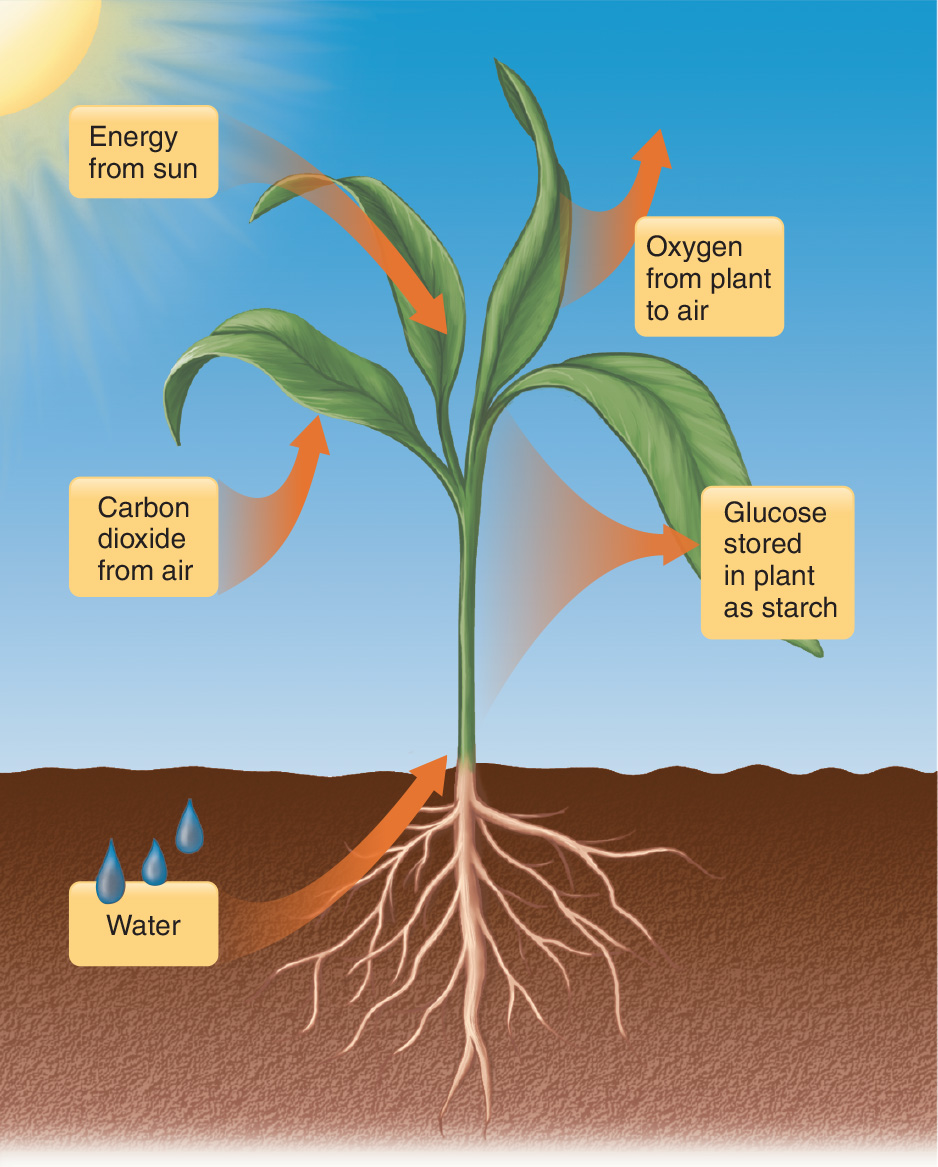
\includegraphics[width=\textwidth]{4_photosynthesis}
	\caption{Photosynthesis}
	\label{fig:photosynthesis}
\end{figure}

Simple carbohydrates contain one or two molecules
\begin{description}
	\item[Monosaccharides] contain only one molecule
	\begin{itemize}
		\item Glucose, fructose, galactose, ribose
	\end{itemize}
	\item[Disaccharides] contain two molecules
	\begin{itemize}
		\item Lactose, maltose, sucrose
	\end{itemize}
\end{description}

\begin{figure}[H]
	\centering
	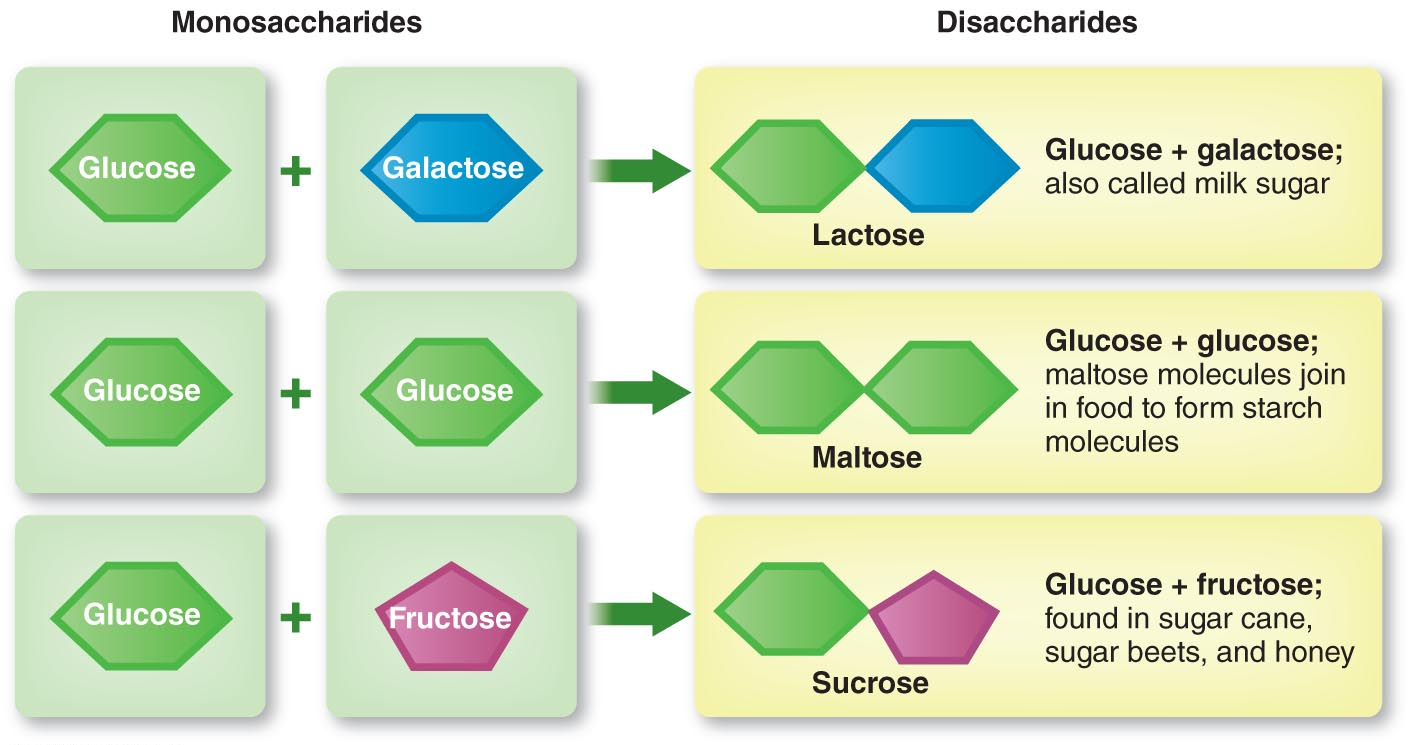
\includegraphics[width=\textwidth]{4_disaccharides}
	\caption{Disaccharides}
	\label{fig:disaccharides}
\end{figure}

\begin{figure}[H]
	\centering
	\begin{subfigure}[b]{0.3\textwidth}
		\centering
		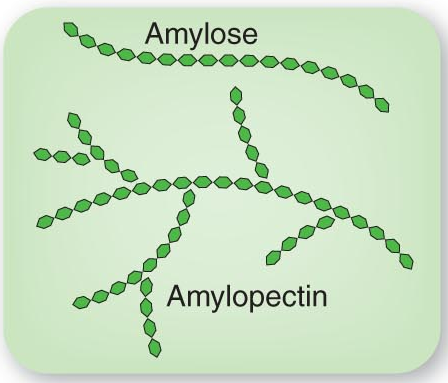
\includegraphics[width=\textwidth]{4_starch}
		\caption{\definition{Starch}{Storage form of glucose in plants; found in grains, legumes, and tubers}}
		\label{fig:starch}
	\end{subfigure}
	\begin{subfigure}[b]{0.3\textwidth}
		\centering
		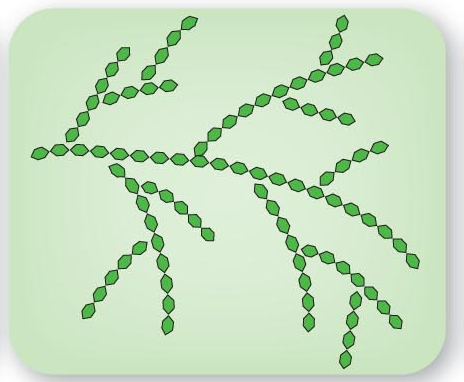
\includegraphics[width=\textwidth]{4_glycogen}
		\caption{\definition{Glycogen}{Storage form of glucose in animals; stored in liver and muscles}}
		\label{fig:glycogen}
	\end{subfigure}
	\begin{subfigure}[b]{0.3\textwidth}
		\centering
		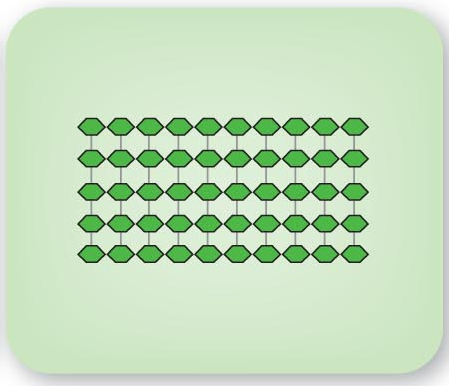
\includegraphics[width=\textwidth]{4_fiber}
		\caption{\definition{Fiber}{Forms the support structures of leaves, stems, and plants}}
		\label{fig:fiber}
	\end{subfigure}
	\caption{Complex Carbohydrates}
	\label{fig:complex-carbohydrates}
\end{figure}

\subsection{Starch}\label{subsec:starch}
\begin{itemize}
	\item Plants store glucose as polysaccharides in the form of starch
	\item Our cells cannot use complex starch molecules exactly as they occur in plants
	\item We digest (break down) starch into glucose
	\item Grains, legumes, and tubers are good sources of dietary starch
\end{itemize}

\subsection{Glycogen}\label{subsec:glycogen}
\begin{itemize}
	\item Animals store glucose as glycogen
	\item Stored in our bodies in the liver and muscles
	\item Not found in food and therefore not a dietary source of carbohydrate
\end{itemize}

\subsection{Fiber}\label{subsec:fiber}
\begin{description}
	\item[Dietary fiber] the non-digestible part of plants
	\begin{itemize}
		\item Also classified by solubility
	\end{itemize}
	\item[Functional fiber] the non-digestible form of carbohydrate with known health benefits, which is extracted from plants and added to foods
	\begin{itemize}
		\item Cellulose, guar gun, pectin, psyllium
	\end{itemize}
	\item[Total fiber] dietary + function fiber
\end{description}

\subsubsection{Soluble fiber}\label{subsubsec:soluble-fiber}
\begin{itemize}
	\item Dissolves in water
	\item Viscous and fermentable
	\item Easily digested by bacteria in the colon
	\item Found in citrus fruits, berries, oats and beans
	\item Reduce risk of cardiovascular disease and type 2 diabetes by lowering blood cholesterol and glucose levels
\end{itemize}

\subsubsection{Insoluble fiber}\label{subsubsec:insoluble-fiber}
\begin{itemize}
	\item Generally do not dissolve in water
	\item Found in whole grains (e.g., wheat, rye, brown rice) and many vegetables
	\item Promote regular bowel movements, alleviate constipation, and reduce risk of diverticulosis
\end{itemize}

\section{Why Do We Need Carbohydrates}\label{sec:why-do-we-need-carbohydrates}
\subsection{Energy}\label{subsec:energy}
\begin{itemize}
	\item Fuel daily activity
	\item Fuel exercise
	\item Help preserve protein for other uses
	\begin{itemize}
		\item When the diet does not provide enough carbohydrates, the process of gluconeogenesis\label{dfn:gluconeogenesis} converts proteins in blood and tissue into glucose
	\end{itemize}
	\item Each gram of carbohydrate = 4 kcal
	\item Red blood cells rely \emph{only} on glucose for their energy supply
	\item Both carbohydrates and fats supply energy for daily activities
	\item Glucose is especially important for energy during exercise
	\item Sufficient energy intake from carbohydrates prevents production of ketones\label{dfn:ketones} as an alternative energy source
	\item Excessive ketones can result in high blood acidity and ketoacidosis
	\item High blood acidity damages body tissues
\end{itemize}

\begin{figure}[H]
	\centering
	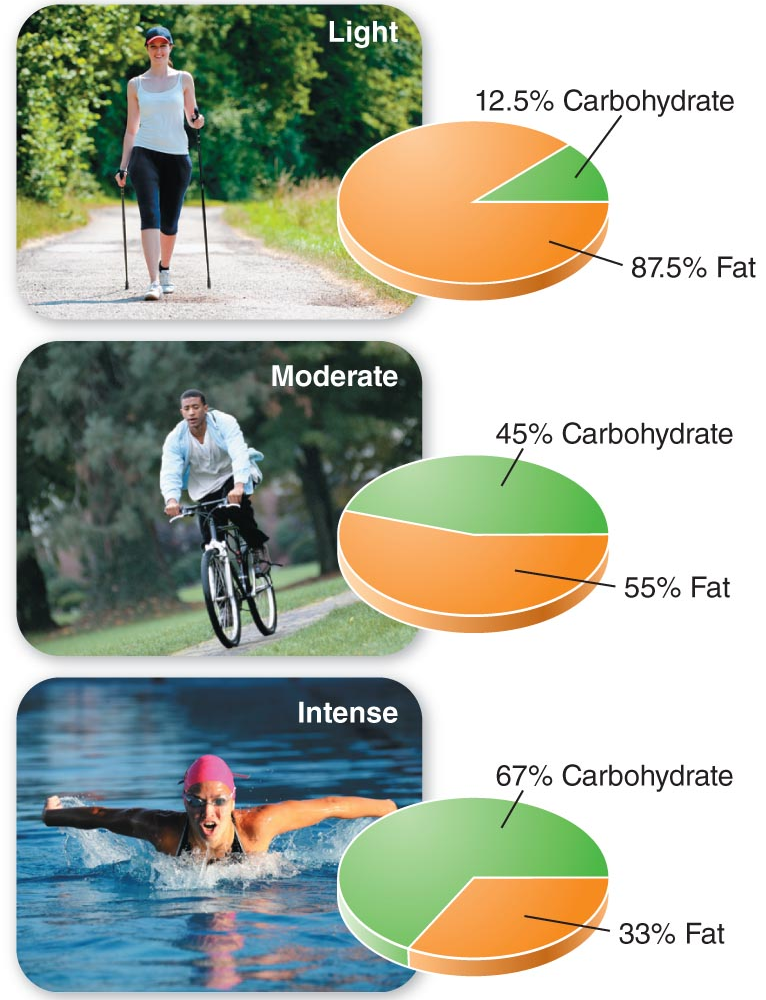
\includegraphics[width=\textwidth]{4_energy_intensity}
	\caption{Carbohydrate Use by Exercise Intensity}
	\label{fig:carb-energy-intensity}
\end{figure}

\subsection{Fiber}\label{subsec:why-we-need-fiber}
\begin{itemize}
	\item May reduce the risk of colon cancer
	\item Promotes bowel health by helping to prevent hemorrhoids and constipation
	\item May reduce the risk of heart disease
	\item May enhance weight loss
	\item May lower the risk of type 2 diabetes
	\item Reduces risk of diverticulosis
\end{itemize}

\begin{figure}[H]
	\centering
	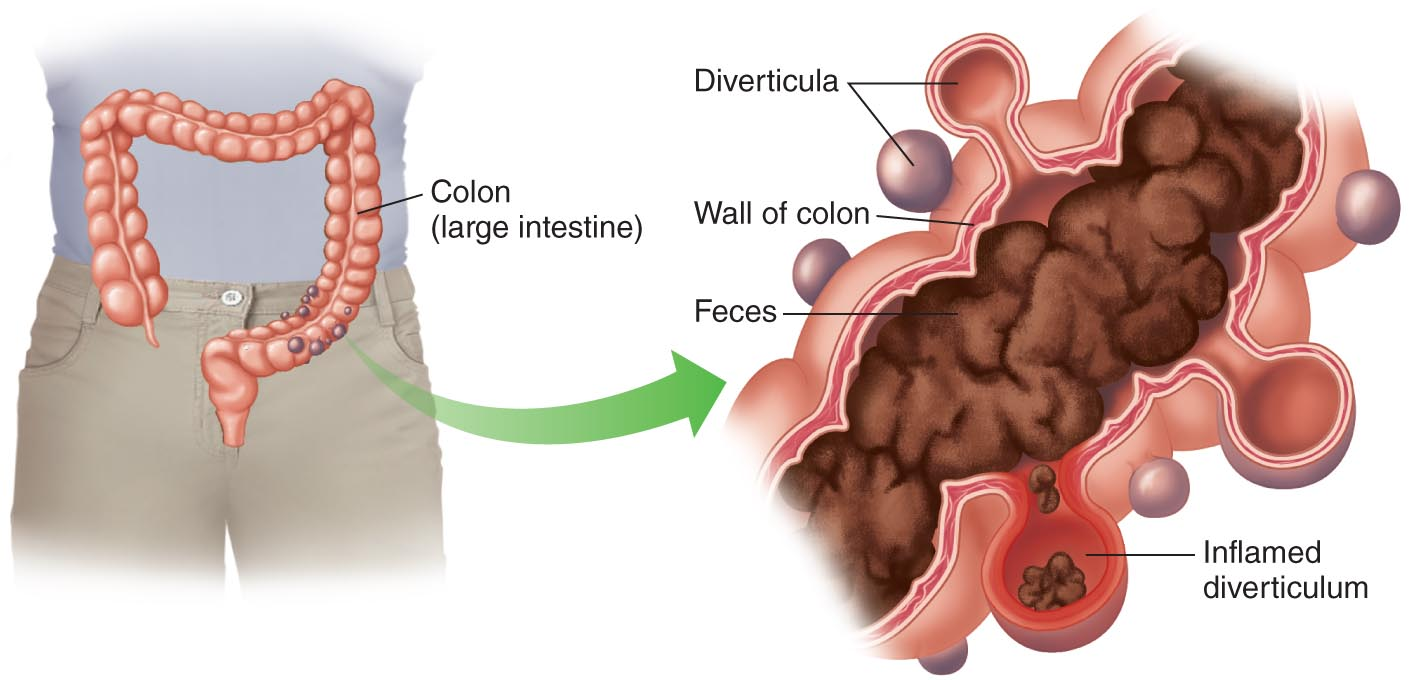
\includegraphics[width=\textwidth]{4_diverticulosis}
	\caption{Diverticulosis}
	\label{fig:diverticulosis}
\end{figure}

\begin{figure}[H]
	\centering
	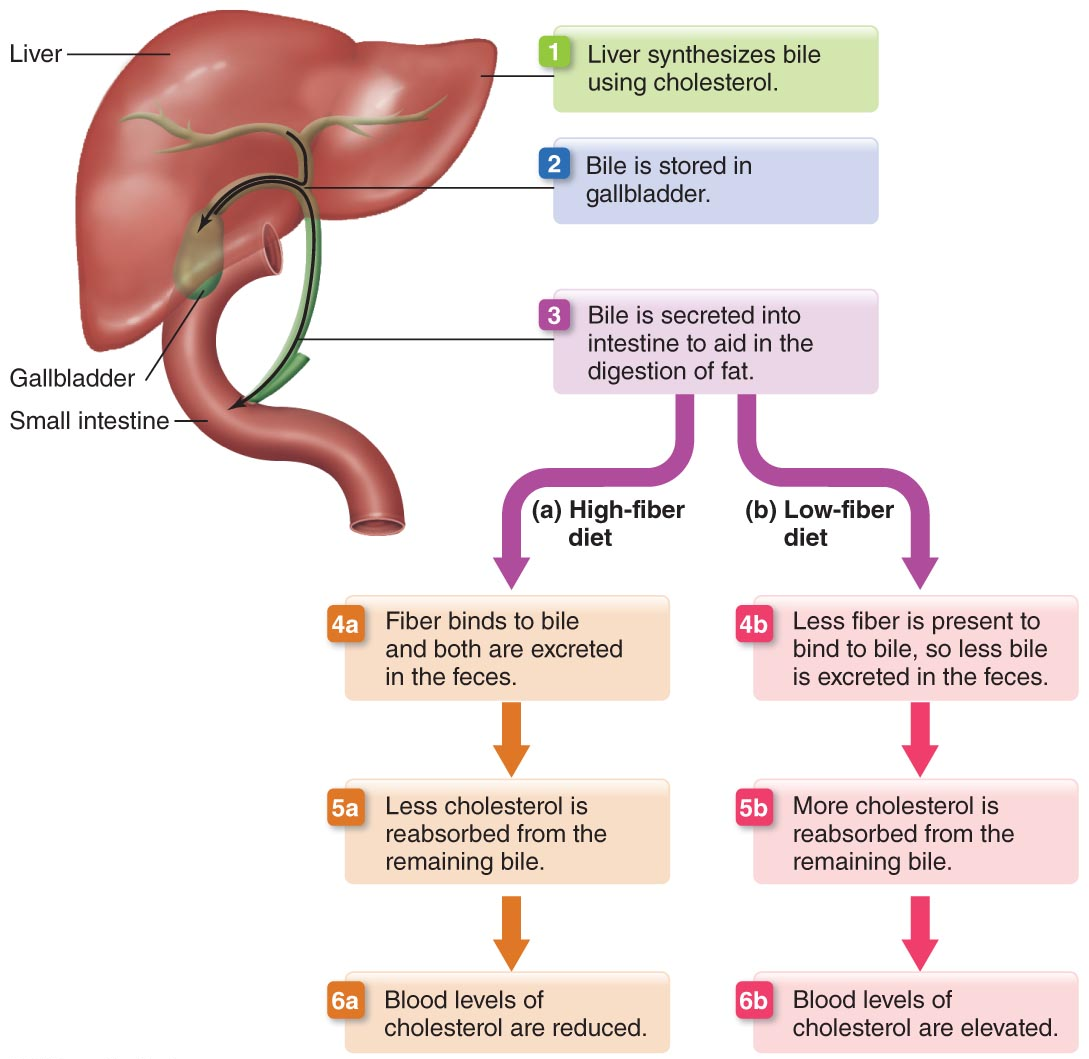
\includegraphics[width=\textwidth]{4_blood_cholesterol}
	\caption{Fiber May Help Decrease Blood Cholesterol}
	\label{fig:fiber-blood-cholesterol}
\end{figure}

\section{Digestion of Carbohydrates}\label{sec:digestion-of-carbohydrates}
\begin{itemize}
	\item Most chemical digestion of carbohydrates occurs in the small intestine
\end{itemize}

\subsection{Pancreatic amylase}\label{subsec:pancreatic-amylase}
\begin{itemize}
	\item Enzyme produced in the pancreas and secreted into the small intestine
	\item Enzymatically digests starch to maltose
\end{itemize}

\begin{itemize}
	\item Additional enzymes secreted by cells that line the small intestine (mucosal cells) digest disaccharides to monosaccharides
	\item These enzymes include maltase, sucrase, and lactase
	\item Monosaccharides are absorbed into the cells lining the small intestine and then enter the bloodstream
	\item Most monosaccharides are converted to glucose by the liver
	\begin{itemize}
		\item Glucose is released into the bloodstream to provide immediate energy
		\item Excess glucose is converted to glycogen and stored in the liver and muscles
	\end{itemize}
\end{itemize}

\begin{figure}[H]
	\centering
	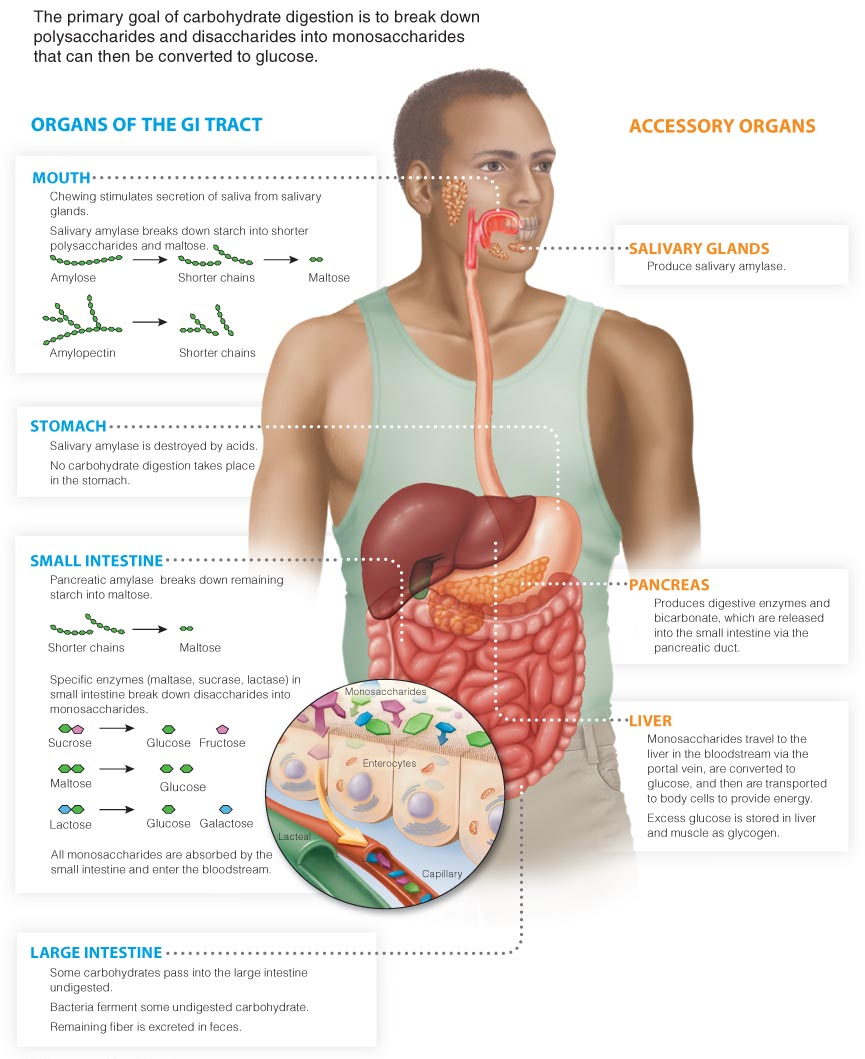
\includegraphics[width=\textwidth]{4_carb_digestion}
	\caption{Digestion of Carbohydrates}
	\label{fig:digestion-of-carbohydrates}
\end{figure}

\section{Regulation of Blood Glucose}\label{sec:regulation-of-blood-glucose}
\subsection{Insulin}\label{subsec:regulation-of-blood-glucose-insulin}
\begin{itemize}
	\item A hormone secreted by the pancreas
	\item Transported in our blood throughout the body
	\item Helps transport glucose from the blood into cells
	\item Stimulates the liver and muscles to take up glucose and convert it to glycogen
\end{itemize}

\begin{figure}[H]
	\centering
	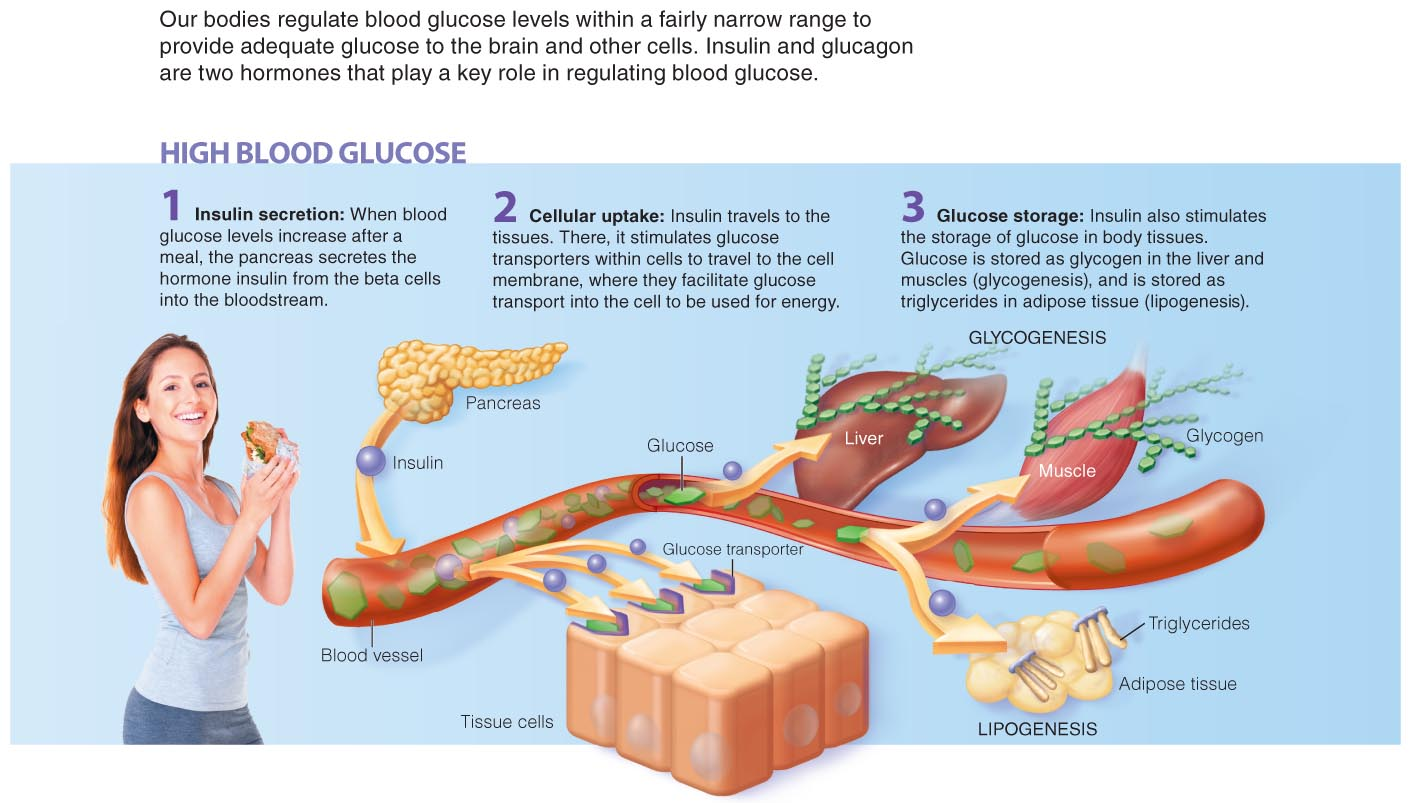
\includegraphics[width=\textwidth]{4_regulation_insulin}
	\caption{Regulation of Blood Glucose: Insulin}
	\label{fig:Regulation-of-Blood-Glucose-Insulin}
\end{figure}

\subsection{Glucagon}\label{subsec:regulation-of-blood-glucose-glucagon}
\begin{itemize}
	\item Another hormone secreted by the pancreas
	\item Stimulates the breakdown of glycogen to glucose to make glucose available to cells of the body
	\item Stimulates gluconeogensis\label{dfn:gluconeogensis}--the production of ``new'' glucose from amino acids
\end{itemize}

\begin{figure}[H]
	\centering
	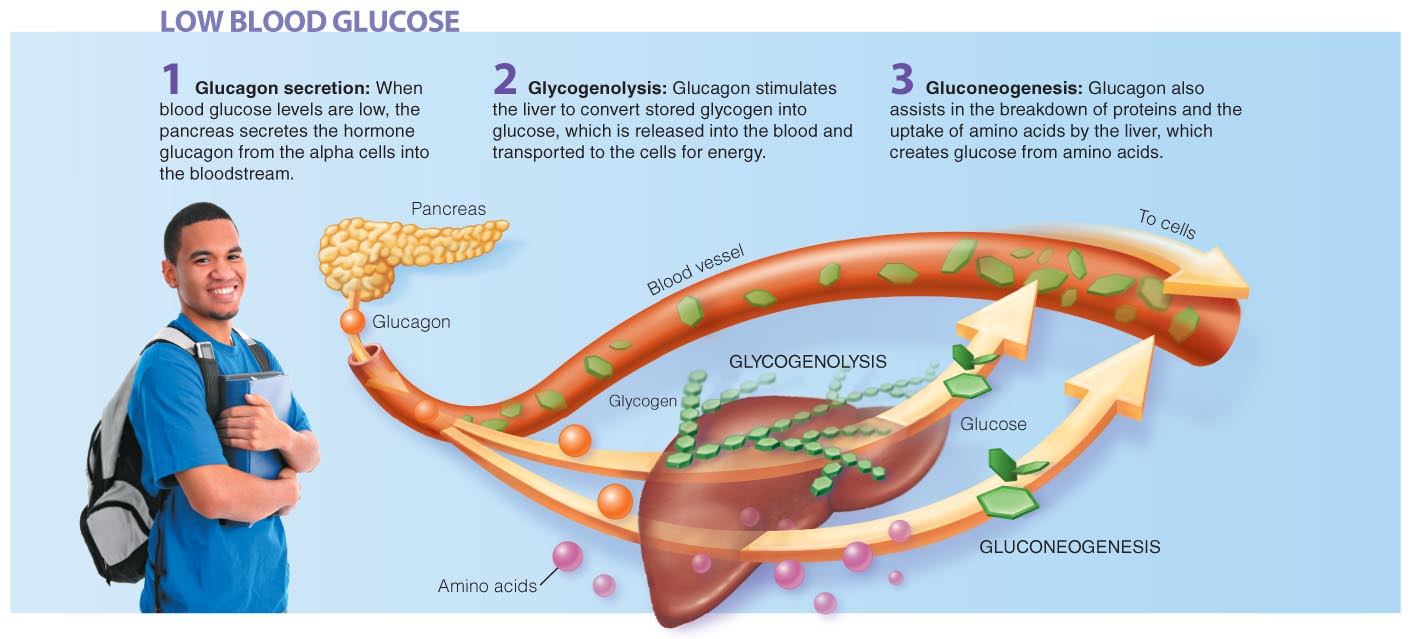
\includegraphics[width=\textwidth]{4_regulation_glucagon}
	\caption{Regulation of Blood Glucose: Glucagon}
	\label{fig:Regulation-of-Blood-Glucose-Glucagon}
\end{figure}

\begin{itemize}
	\item Fructose does not stimulate the release of insulin
	\begin{itemize}
		\item Fructose is metabolized differently then glucose
		\item Absorbed further down in the small intestine
	\end{itemize}
\end{itemize}

\begin{description}
	\item[Glycemic index] a measure of a food's ability to raise blood glucose levels
	\begin{itemize}
		\item Foods wih a low glycemic index cause low to moderate fluctuations in blood glucose
	\end{itemize}
	\item[Glycemic load] amount fo carbohydrate in a food multiplied by its glycemic index
	\begin{itemize}
		\item Considered a more useful tool than glycemic index
	\end{itemize}
\end{description}

\begin{figure}[H]
	\centering
	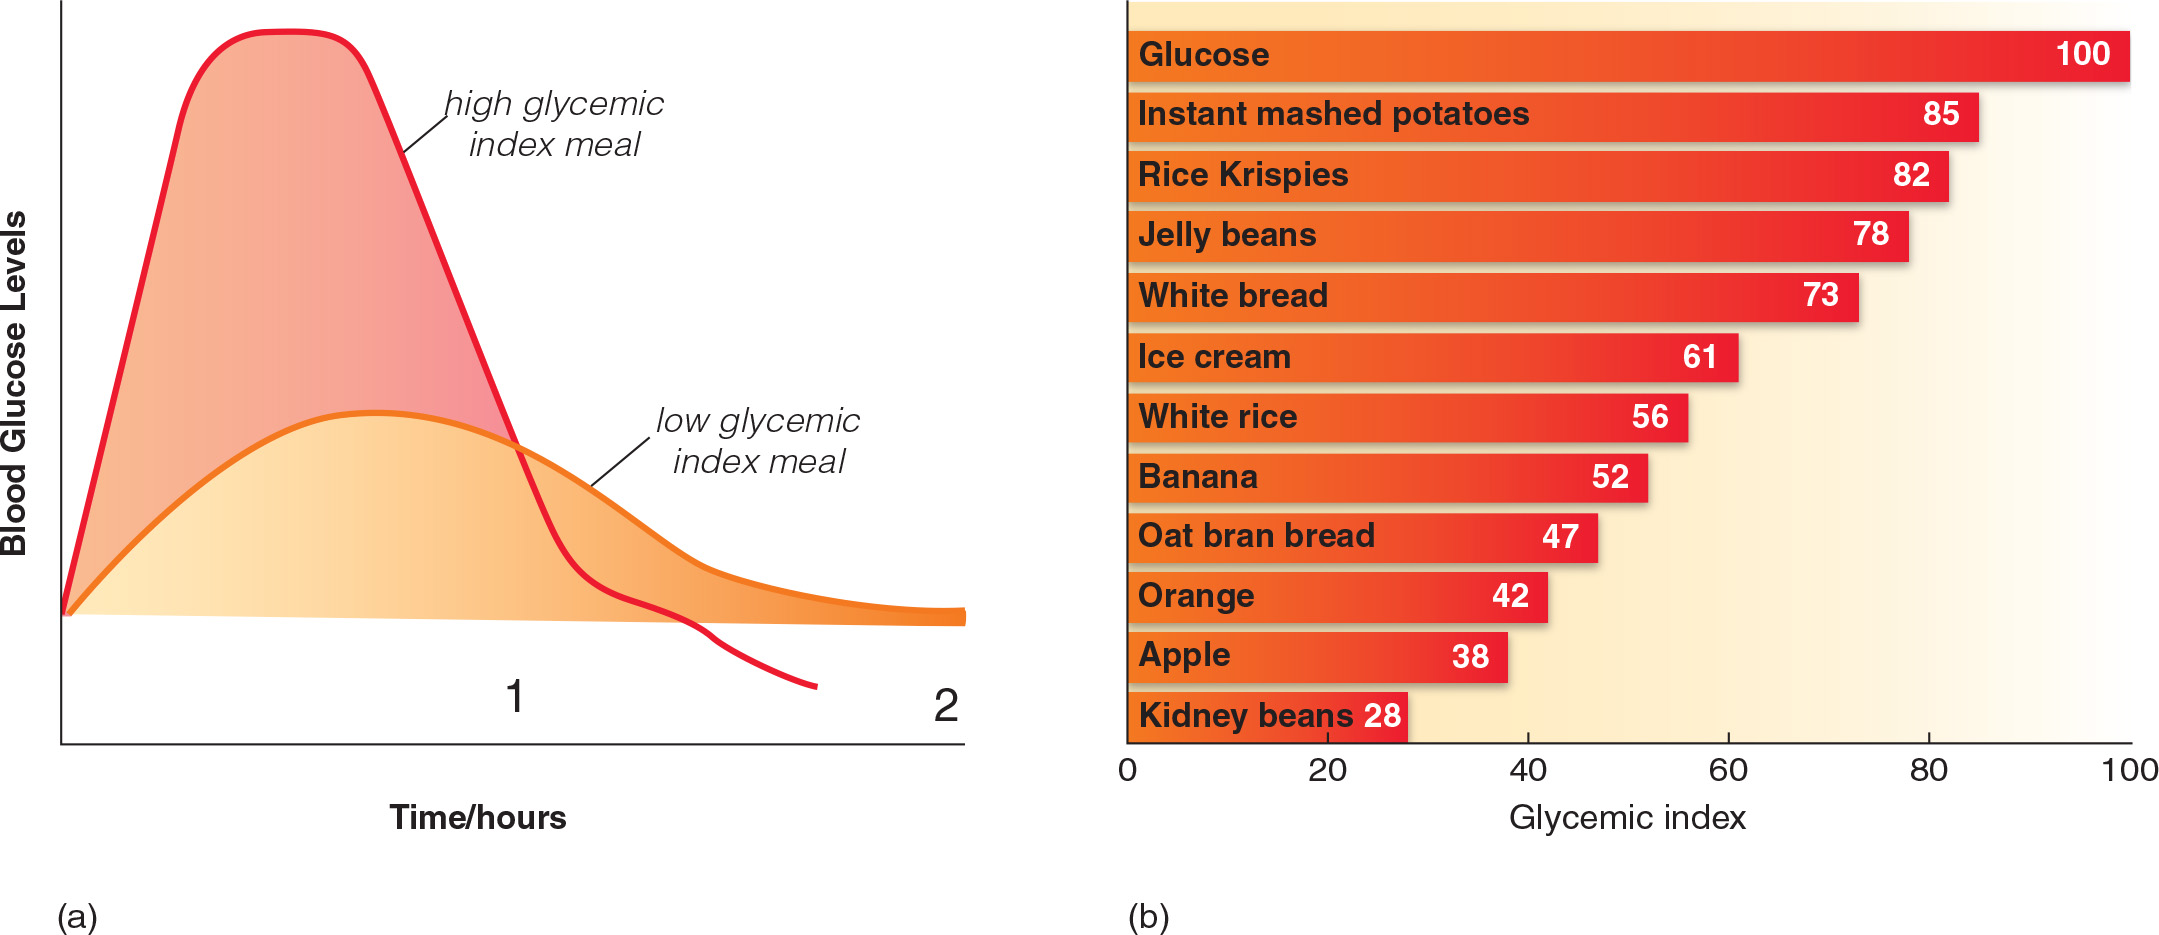
\includegraphics[width=\textwidth]{4_regulation_glucose}
	\caption{Regulation of Blood Glucose}
	\label{fig:Regulation-of-Blood-Glucose}
\end{figure}

\begin{itemize}
	\item Foods and meals with a lower glycemic load
	\begin{itemize}
		\item Are better for people with diabetes
		\item Are generally higher in fiber
		\item May reduce the risk of heart disease and colon cancer
		\item Are associated with a reduced risk of prostate cancer
	\end{itemize}
\end{itemize}

\section{How Much Carbohydrate Should We Eat?}\label{sec:how-much-carbohydrate-should-we-eat?}
\begin{itemize}
	\item The Recommended Dietary Allowance (RDA) for carbohydrate is 130 g per day just to supply the brain with glucose
	\begin{itemize}
		\item 45--65\% of daily Calorie intake should be in the form of carbohydrates
		\item Focus on foods high in fiber and low in added sugars
	\end{itemize}
	\item Most Americans eat too much added sugar
	\begin{itemize}
		\item Sugars are added to foods during processing or preparation
		\item Most common source is soft drinks
		\item Typical sources are cookies, candy, fruit drinks
		\item Unexpected sources include peanut butter, flavored rice mixes, salad dressing
		\item Added sugars are not chemically different from naturally occurring sugars, but have fewer vitamins
	\end{itemize}
	\item Sugars are blamed for many health problems
	\begin{itemize}
		\item Can cause dental problems and tooth decay
		\item No proven association with childhood hyperactivity; long-term effects not known
		\item Associated with increased ``bad cholesterol'' and decreased ``good cholesterol''
		\item Associated with a higher risk of diabetes
		\item Associated with obesity
	\end{itemize}
	\item Most Americans eat too little fiber-rich carbohydrates
	\item The Adequate Intake (AI) of fiber is 14 grams per 1,000 kcal in the diet daily (or 25 g for women; 38 g for men)
	\item Whole-grain foods (grains, vegetables, fruits, nuts, legumes) are much more healthful sources than foods with added sugar or fiber
	\begin{itemize}
		\item Whole grains are kernels that retain the bran, endosperm, and germ
	\end{itemize}
\end{itemize}

\begin{figure}[H]
	\centering
	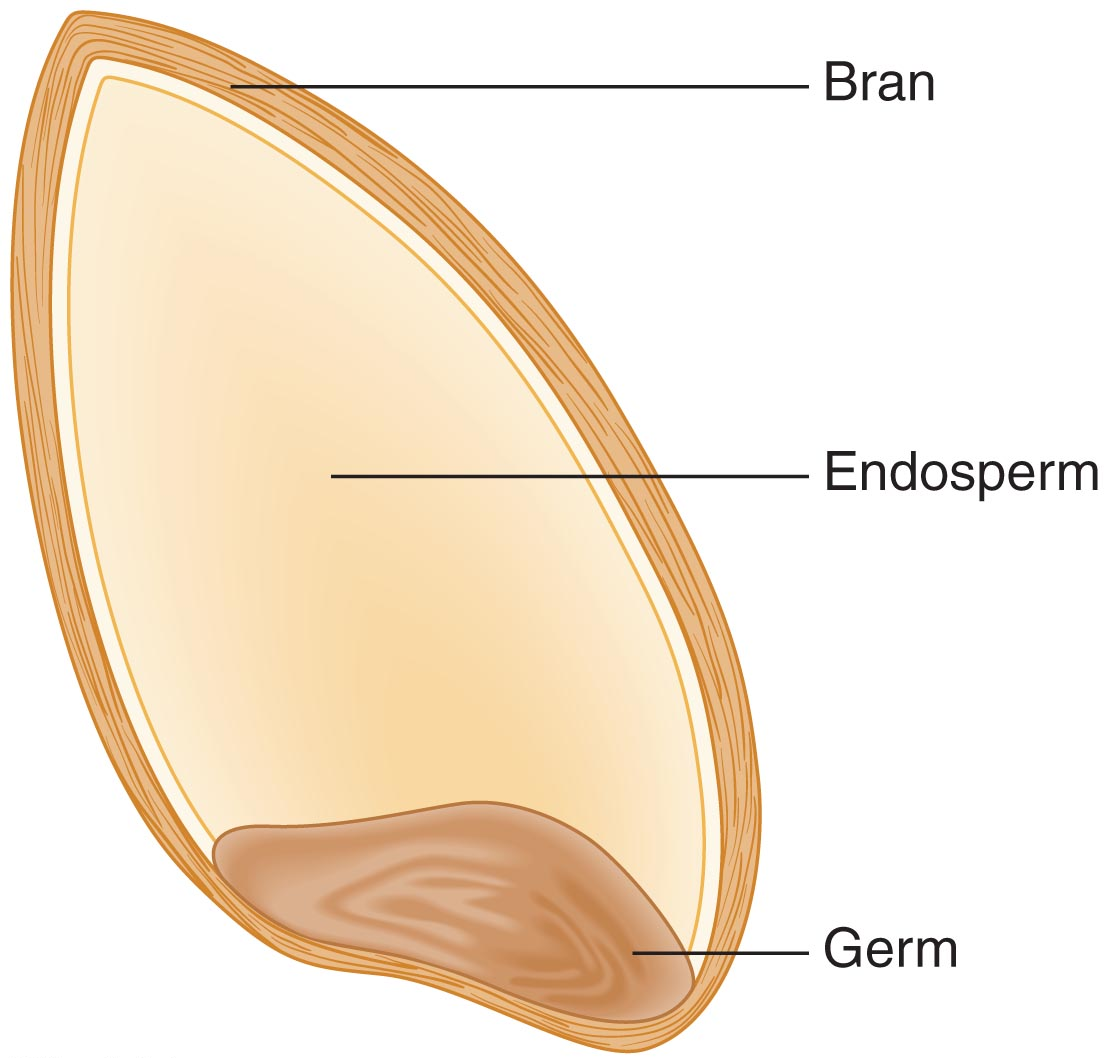
\includegraphics[width=\textwidth]{4_whole_grain}
	\caption{Whole Grain}
	\label{fig:whole-grain}
\end{figure}


\begin{table}[H]
    \centering
    \begin{threeparttable}
		\caption{Dietary Recommendations for Carbohydrates}
		\label{tab:dietary-recommendations-for-carbohydrates}
		\begin{tabular}{>{\columncolor{rowlightgreen}}p{0.475\textwidth} >{\columncolor{rowmedgreen}}p{0.475\textwidth}}
			\rowcolor{rowdarkgreen}\textbf{Health and Medicine Division of the National Academies of Science Recommendations*} & \textbf{2015--2020 Dietary Guidelines for Americans\textdagger}\\
				Recommended Dietary Allowance (RDA) for adults 19 years of age and older is 130 g of carbohydrate per day.

				The \hyperref[subsec:amdr]{Acceptable Macronutrient Distribution Range (AMDR)} for carbohydrate is 45--65\% of total daily energy intake.

				Added sugar intake should be 25\% of less of total energy intake each day. &
				Consume a healthful eating pattern that accounts for all foods and beverages within an appropriate Calorie level.
				A healthful eating pattern includes: a variety of vegetables from all subgroups (dark green, red and orange, legumes, starch and other); fruits (especially whole fruits); grains (at least half of which are whole grains); fat-free or low-fat dairy; a variety of protein foods; and oils.\\
			\rowcolor{rowdarkgreen} & \\
		\end{tabular}
		\begin{tablenotes}
			\small
			\item *Data from:
		\end{tablenotes}
	\end{threeparttable}
\end{table}

%\makebox[\t/extwidth][c]{
\begin{table}[H]
    \centering
	\begin{adjustbox}{max width=0.975\paperwidth,center}
		\begin{threeparttable}
			\caption{Forms of Sugar Commonly Added to Foods}
			\label{tab:forms-of-sugar commonly-added-to-foods}
			\rowcolors{2}{rowmedgreen}{rowlightgreen}
			\begin{tabular}{p{0.4\textwidth} p{0.7\textwidth}}
				\rowcolor{rowdarkgreen}\textbf{Name of Sugar} & \textbf{Definition}\\
				Brown sugar & A highly refined sweetener made up approximately 99\% sucrose and produced by adding to white table sugar either molasses or burnt table sugar for clothing and flavor.\\
				Cane sugar & Sucrose that has been extracted from sugarcane, a tropical plant naturally rich in sugar.\\
				Concentrated fruit juice sweetener & A form of sweetener made with concentrated fruit juice, commonly pear juice.\\
				Confectioner's sugar & A highly refined, finely ground white sugar; also referred to as powdered sugar. \\
				Corn sweeteners & A general term for any sweetener made with corn starch\\
				Corn syrup & A syrup produced by the partial hydrolysis of corn starch.\\
				Dextrose & An alternative term for glucose.\\
				Fructose & A monosaccharide that occurs in fruits and vegetables; also called levulose, or fruit sugar.\\
				Galactose & A monosaccharide that joins with glucose to create lactose.\\
				Granulated sugar & Another term for white sugar, or table sugar.\\
				High-fructose corn syrup & A type of corn in which part of the sucrose is converted to fructose, making it sweeter than sucrose or regular corn syrup; most high-fructose corn syrup contains 42\% to 55\% fructose. \\
				Honey & A sweet, sticky liquid sweetener made by bees from the nectar of flowers; contains glucose and fructose.\\
				Invert sugar & A sugar created by heating a sucrose syrup with a small amount of acid; inverting sucrose results in its breakdown into glucose and fructose, which reduces the size of the sugar crystals; because of its smooth texture, it is used in making candies and some syrups.\\
				Levulose & Another term for fructose, or fruit sugar.\\
				Mannitol & A type of sugar alcohol\\
				Maple sugar & A sugar made by boiling maple syrup\\
				Molasses & A thick, brown syrup that results from the processing of sugar beets or sugarcane; it is approximately 96\% to 98\% sucrose; true raw sugar contains impurities and is not stable in storage; the raw sugar available to consumers has been purified to yield an edible sugar.\\
				Natural sweeteners & A general term used for any naturally occurring sweeteners, such as fructose, honer, and raw sugar.\\
				Raw sugar & The sugar that results from the processing of sugar beets or sugarcane; it is approximately 96\% to 98\% sucrose; true raw sugar contains impurities and is not stable in storage; the raw sugar available to consumers has been purified to yield an edible sugar.\\
				Sorbitol & A type of sugar alcohol\\
				Turbinado sugar & The form of raw sugar that is purified and safe for human consumption; sold as ``Sugar in the Raw'' in the United States.\\
				White sugar & Another name for sucrose, or table sugar.\\
				Xylitol & A type of sugar alcohol\\
				\rowcolor{rowdarkgreen} & \\
			\end{tabular}
			\begin{tablenotes}
				\small
				\item
			\end{tablenotes}
		\end{threeparttable}
	\end{adjustbox}
\end{table}

\section{Alternative Sweeteners}\label{sec:alternative-sweeteners}
\subsection{Nutritive sweeteners}\label{subsec:nutritive-sweeteners}
\begin{itemize}
	\item Contain 4 kcal energy per gram
	\item Sucrose, fructose, honey, brown sugar
\end{itemize}

\subsection{Sugar alcohols}\label{subsec:sugar-alcohols}
\begin{itemize}
	\item Contain 2--3 kcal energy per gram
	\item Have the benefit of a decreased glycemic response and decreased risk of dental caries
\end{itemize}

\subsection{Non-nutritive (alternative) sweeteners}\label{subsec:non-nutritive-(alternative)-sweeteners}
\begin{itemize}
	\item Provide little or no energy
	\item Developed to sweeten foods without the usual risks
\end{itemize}

\begin{itemize}
	\item No Acceptable Daily Intake (ADI) has been set for saccharin (e.g., ``Sweet n' Low''), but it has been removed from the list of cancer-causing agents
	\item ADIs have been established for
	\begin{description}
		\item[Acesulfame-K] ``Sweet One'', ``Sunette''
		\item[Aspartame] ``Equal''
		\item[Sucralose] ``Splenda''
	\end{description}
\end{itemize}

\section{Diabetes}\label{sec:diabetes}
\begin{itemize}
	\item Inability to regulate blood glucose levels
	\item \definition{Hyperglycemia}{in which glucose levels are higher than normal--becomes chronic}
	\item Three types
	\begin{itemize}
		\item Type 1 diabetes
		\item Type 2 diabetes
		\item Gestational diabetes
	\end{itemize}
	\item Uncontrolled diabetes can cause infections, nerve damage, kidney damage, blindness, seizures, stroke, and cardiovascular disease; and can be fatal
\end{itemize}

\subsection{Type 1 Diabetes}\label{subsec:type-1-diabetes}
\begin{itemize}
	\item Accounts for about 5\% of all cases
	\item Body does not produce enough insulin
	\item Creates high blood sugar (glucose) levels
	\item Key warning sign is frequent urination
	\item May lead to ketoacidosis, coma and death
	\item Classified as an autoimmune disease
	\item Most frequently diagnosed in adolescents
	\item Has a genetic link
\end{itemize}

\subsection{Type 2 Diabetes}\label{subsec:type-2-diabetes}
\begin{itemize}
	\item Accounts for 90--95\% of cases
	\item Develops progressively over time
	\item Body cells become insensitive or unresponsive to insulin
	\item Obesity is most common trigger
	\item Variations include insulin resistance, impaired fasting glucose, and pre-diabetes
	\item Eventually the pancreas may become unable to produce any insulin
\end{itemize}

\section{Diabetes Testing and Diagnosis}\label{sec:diabetes-testing-and-diagnosis}
\begin{itemize}
	\item Three blood tests can be used to diagnose diabetes
	\begin{itemize}
		\item Fasting plasma glucose (FPG)
		\item Oral glucose tolerance (OGT)
		\item Glycosylated hemoglobin test (HbA1c)
	\end{itemize}
\end{itemize}

\begin{figure}[H]
	\centering
	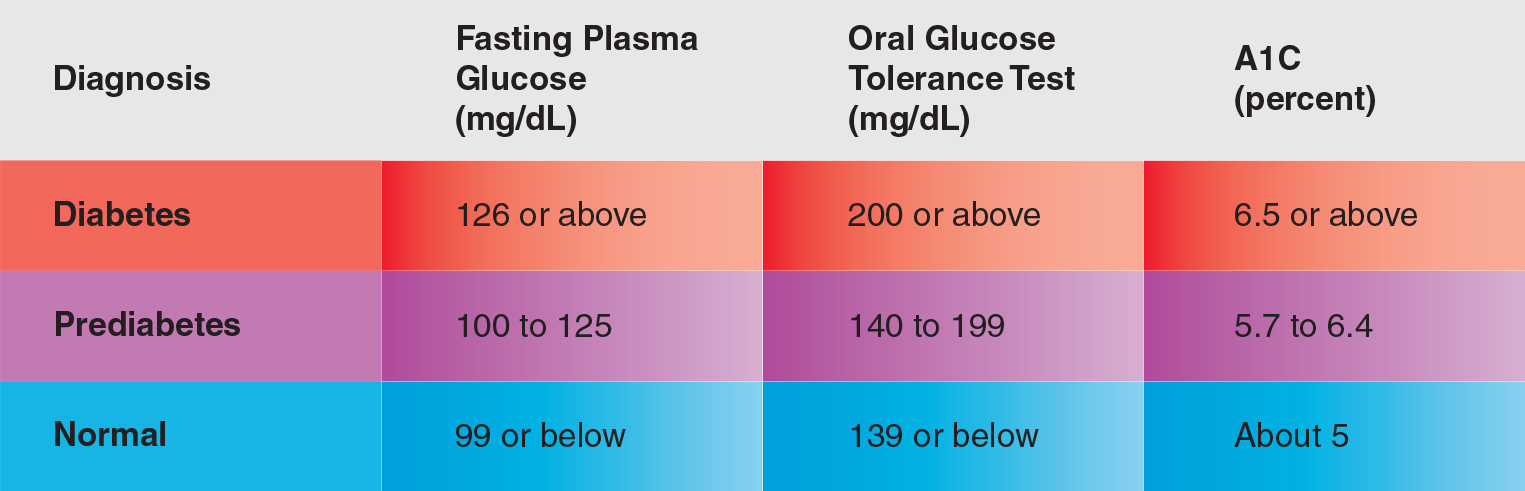
\includegraphics[width=\textwidth]{4_diabetes_diagonsis}
	\caption{Diabetes Testing and Diagnosis}
	\label{fig:diabetes-testing-and-diagnosis}
\end{figure}

\subsection{Who is at risk?}\label{subsec:who-is-at-risk?}
\begin{itemize}
	\item Obesity, genetics, physical inactivity, and poor diet increase overall risk
	\item Metabolic syndrome (high waist circumference, high blood pressure, high blood lipids and glucose) increases risk of type 2 diabetes
	\item Increased age increases risk, but younger people and children are now commonly diagnosed
\end{itemize}

\subsection{Prevention and control}\label{subsec:prevention-and-control}
\begin{itemize}
	\item Eat a healthful diet, get daily exercise, keep a healthful body weight
	\item Limit intake of added sugars
	\item Choose fiber-rich foods like whole grains
	\item Limit consumption of red meat and processed meat
	\item Avoid alcoholic beverages, which can cause hypoglycemia
	\item Healthful lifestyle choices can prevent or delay onset of type 2 diabetes
	\item Oral medications and/or insulin injections may be required once diabetes has been diagnosed
\end{itemize}

%</Chapter4>

\end{document}
